\documentclass[10pt, a4paper]{article}

% Formatting
\usepackage{ctex}
\usepackage[margin=1in]{geometry}
\usepackage[titletoc,title]{appendix}

\usepackage[colorlinks,linkcolor=red]{hyperref}
\usepackage{amsmath,amsfonts,amssymb,mathtools}


\usepackage{graphicx,float}
\usepackage{xcolor}

\usepackage[ruled,vlined]{algorithm2e}
\usepackage{algorithmic}


\everymath{\displaystyle}


\usepackage{biblatex}
\addbibresource{references.bib}

% Title content
\title{数理统计学习笔记8-9}
\author{慕弋云子}
\date{November 7, 2020}

\begin{document}
\setcounter{section}{7}
\maketitle

写这些东西主要是为了:
\begin{enumerate}
    \item 对于期末突击的同学们,可以迅速把握考点和做题技巧。
    \item 对于保研的同学、或者已经忘了概统内容甚至完全没学过的同学,这是一份很好的补充材料。
    \item 对于历年新生,可以做到不必听课,独立阅读文档并认真完成老师留的作业,就可以很好地完成数理统计的学习。
\end{enumerate}

阅读本文前你需要知道:
\begin{enumerate}
    \item 本人是2020级孙海燕老师班的学生,首先必须声明的是,孙老师讲得挺好的,对于许多概念有着深厚的理解和把握,授课思路也很清晰,但大抵是要照顾各种程度的学生,所以进度对于我这样的考研学生就显得有些“食之无味,弃之可惜”。于是,我便解锁了边听课边写作业的操作,争取每周形成此文,带领大家巩固每周的内容并更好地完成作业。
    \item 数理统计本身的知识内容就有很强的抽象性,配合北航这形式化的教材,自学起来实在困难。所以我们不如找一个生动形象、轻松诙谐的方式,来共同完成一些概念的学习。在这个过程中可能不那么严谨,但会更加直观。
    \item 本文内容都是基于孙老师课堂内容及所布置作业,每一大节对应每节课的作业。对于本文未提及的知识点和习题类型,学有余力者可自行学习;本文内容亦不对诸位读者的考试成绩负责,还望知悉。
\end{enumerate}\par

此外,本人对于latex的使用略有生疏,以及对于数理统计知识的掌握难免有疏漏之处,还望见谅。如对本文内容有任何问题,欢迎私信或发邮件至:gt3115a@163.com。\par
另附本文GitHub Repo的地址,在这里你可以找到之前或之后的内容,不会迷路:\url{www.github.com/Muyiyunzi/ShuLiTongJi_BUAA}

\section{相合估计与区间估计}
作业内容参考:2.48、2.50、2.51、2.52\par

之前说上上节的内容是“暴风雨前的宁静”、上节内容是“暴风雨夹雪”,那么这节的内容应该就是“雨后天晴”了。本次的内容非常简单和基础,而且内容也不超过考研的范围,算是用起来比较套路、同时还比较好理解的东西了。\par

同样地,我还是会用尽量生动形象的方式让大家理解抽象的概念,同时总结做题目的套路,大家可以根据自己的情况自取所需。以及,欢迎任何对本文内容的讨论。

\subsection{依……收敛}

在给出相合估计的概念之前,我们还是先来填一填以前的坑。“依……收敛”这样的字眼肯定令不少人头疼,虽然这对于理解之后的不等式、相合估计等内容并不会造成太大影响,但我认为我们还是有必要在这里一起总结一下,目的性比较功利的同学可以跳过本小节。\par
目前主要会接触到四种“依……收敛”,罗列如下:
\subsubsection*{依概率收敛}
关于依概率收敛,我这里的理解可以参见\href{https://www.zhihu.com/question/19911209/answer/876481176}{大数定律具体是个什么概念?}的第一条。这里是基于频率和概率的关系定义的,简言之就是,我们在抛硬币(抽样)的过程中,虽然频率与概率不会完全地重合,但是我们可以画一个足够小的界限$\varepsilon$,使频率不会超越概率两侧的界限$p \pm \varepsilon$。这时我们就称频率依概率收敛为概率。\par
而在试验刚开始的时候,频率当然是可以跨过这个界限的,形象地说,依概率收敛只要求\textbf{“尾巴收敛”}。在形式上,更一般地我们定义$X_{n}$表示统计量(比如频率),定义$X$表示被估计量(如概率),那么依概率收敛的定义应该是:\par
对于$\forall \varepsilon > 0$有:
\begin{center}
    $\lim _{n \rightarrow \infty} P\left\{\left|X_{n}-X\right| \geq \varepsilon\right\}=0$
\end{center} \par
(即越界是小概率事件),或:
\begin{center}
    $\lim _{n \rightarrow \infty} P\left\{\left|X_{n}-X\right| \leq \varepsilon\right\}=1$
\end{center} \par
(即大概率在界内),此二者定义是等价的。



\subsubsection*{依概率1收敛}
与依概率收敛相对地,依概率1收敛要求\textbf{“整体收敛”};在形式上,它把limit放到了概率里边,并直接要求统计量与被估计量相等。这样的条件更强,所以也称\textbf{“几乎必然收敛”},即表示为:
\begin{center}
    $ P\left\{\lim _{n \rightarrow \infty}X_{n}=X \right\}=1$
\end{center}

\subsubsection*{依分布收敛}
相比之下,依分布收敛则是更强的,这要求数据的总体分布直接服从某一特定分布族。在我们所学过的知识中,最典型的代表便是\textbf{中心极限定理}。关于CLT的内容可以同样参见上面的知乎链接第五条,如果对第一篇学习笔记有过阅读的话,想必对CLT应该也有足够的了解,在此不做展开。

\subsubsection*{r阶收敛}
这里直接给出r阶收敛的定义式,不是本节重点所以不做过多赘述。称:
\begin{center}
    $ \lim _{n \rightarrow \infty} E~| X_{n} - X | ^r =0$
\end{center}
为$X_n~$r阶收敛于$X$。\par
研究随机过程、机械振动等较传统工科的同学应该对特定的$r=2$阶收敛,即均方收敛(亦作m. s. 收敛)更加熟悉。

\subsection{相合估计}
相合估计是个很简单的概念,在层次关系上和我们之前学过的无偏估计、有效估计是\textbf{并列}的。其思想也比较朴素,就是希望当样本容量\textbf{趋于无限大}的时候,一个统计量(书中使用的是“估计序列”这个术语,我认为可不做区分)能够\textbf{越来越接近}参数的真实值,这就是相合估计。\par
所以说,如何定义“越来越接近”这件事情就产生了对相合性的子层次定义:
\begin{enumerate}
    \item 如果统计量是\textbf{依概率收敛}于参数真值,称其为\textbf{弱}相合估计。
    \item 如果统计量是\textbf{依概率1收敛}于参数真值,称其为\textbf{强}相合估计。
    \item 如果统计量是\textbf{r阶收敛}于参数真值,称其为\textbf{r阶}相合估计。
\end{enumerate} \par
后两条不重要,我们一般都讨论依概率收敛的弱相合估计。\par
类似我们在学习极限时,描述这种“无穷而又收敛”的情况,引入$\varepsilon-\sigma$语言来形式地描述这件事情,可以直接套用依概率收敛的定义式:\par
对于$\forall \varepsilon > 0$有:
\begin{center}
    $\lim _{n \rightarrow \infty} P_\theta\left\{\left|\hat{q}_n - q(\theta) \right| \geq \varepsilon\right\}=0$
\end{center} \par
实际上我们这里只是把$X_n$替换为了$\hat{q}_n$以表示一个统计量,对应地使用$q(\theta)$表示未知参数的函数。


\subsection{Markov与Chebyshev不等式}
然后有一个问题就是,相合估计定义得看起来如此复杂,我们该怎么去证明某个统计量确实是相合估计、确实依概率收敛呢?这时就可以引入马尔可夫不等式(Markov Inequility)和切比雪夫不等式(Chebyshev Inequility)了。\par
说起这个可以顺便和大家聊聊彼得堡学派。
\begin{figure}[H]
    \centering
    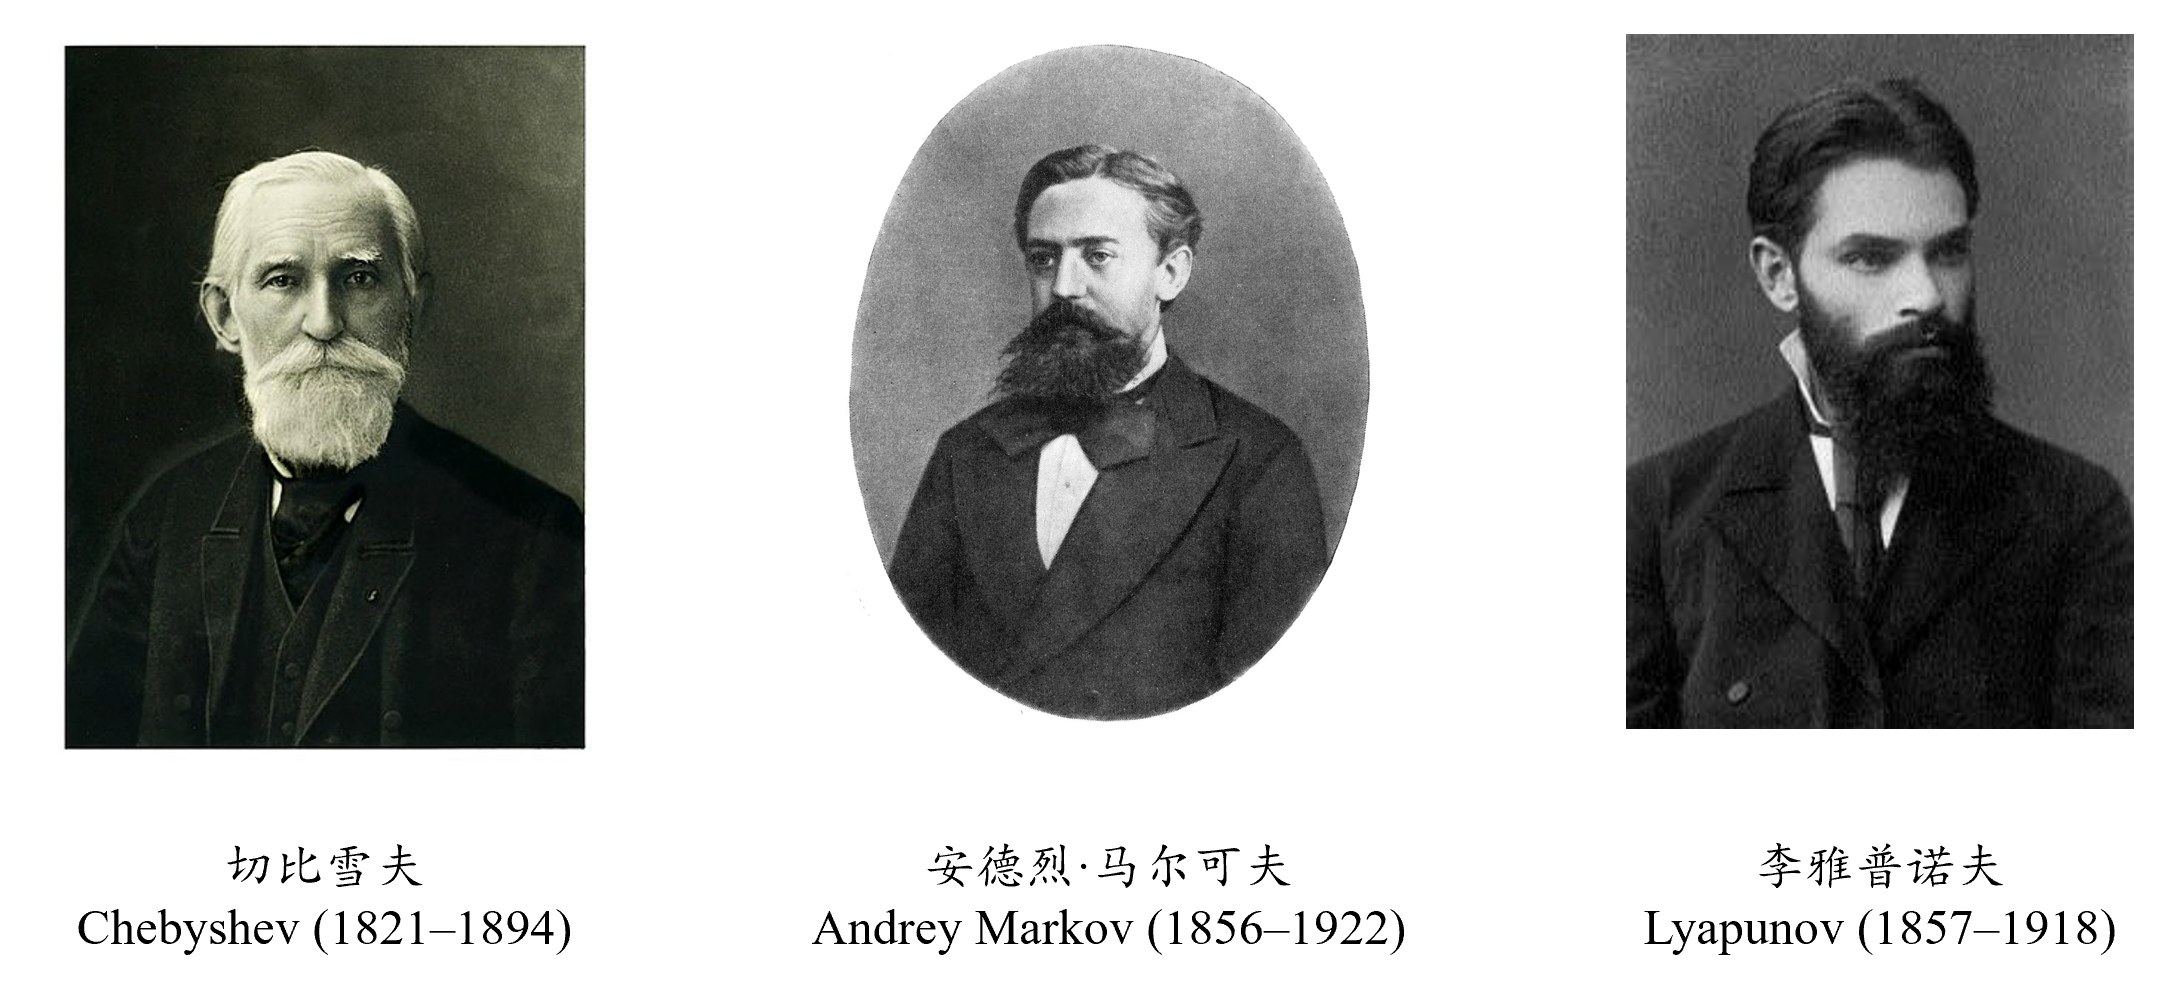
\includegraphics[width=\linewidth]{petersburg.png}
    \caption{彼得堡(Petersburg)学派}
    \label{fig:petersburg}
\end{figure}

最左边这个就是老师切比雪夫,其学生有很多,最有代表性的两位当属马尔可夫和李雅普诺夫,前者更多的贡献是对于随机过程的,比如马尔可夫链、马尔科夫场、隐马模型等等,后者则涉猎广泛,诸如概率论、常微分方程、运动稳定性等,以其名命名的定理、条件等更是数不胜数。\par
也就是从切比雪夫开始,俄罗斯的数学水平突然走到了欧洲前列,与此相对的还有莫斯科学派,那里的人名对大家应该也是耳熟能详的,比如辛钦(大数定律)、柯尔莫哥洛夫(太多贡献说不完)等等……大概这就是底蕴吧。\\ \par
说回到Markov不等式与Chebyshev不等式,这真的令我回想到自己考研的日子,明明进度已经很紧张了,却抱着手机看各种关于这两个不等式的知乎解读。这里尤为推荐姚岑卓的这篇\href{https://www.zhihu.com/question/27821324/answer/80814695}{切比雪夫不等式到底是个什么概念?},里边对于这两个不等式的几何直观理解非常独到。\par
一般Markov不等式都默认指一阶情况,大家可以根据这个回答自行推广到$l$阶Markov不等式,并画出其几何直观图。我这里顺便给出$l$阶Markov不等式的形式化定义,以及我自己画出来的几何直观给大家一个参考:

\subsection*{Markov不等式}
若样本k阶原点矩存在,则对于小于等于k的每一阶原点矩都有,对于$\forall \varepsilon > 0$,有:
\begin{center}
    $P\{|X| \geqslant \varepsilon\} \leqslant \frac{E(|X|^{l} ) }{\varepsilon^{l}}, \quad l=1,2, \cdots, k$
\end{center}


\begin{figure}[H]
    \centering
    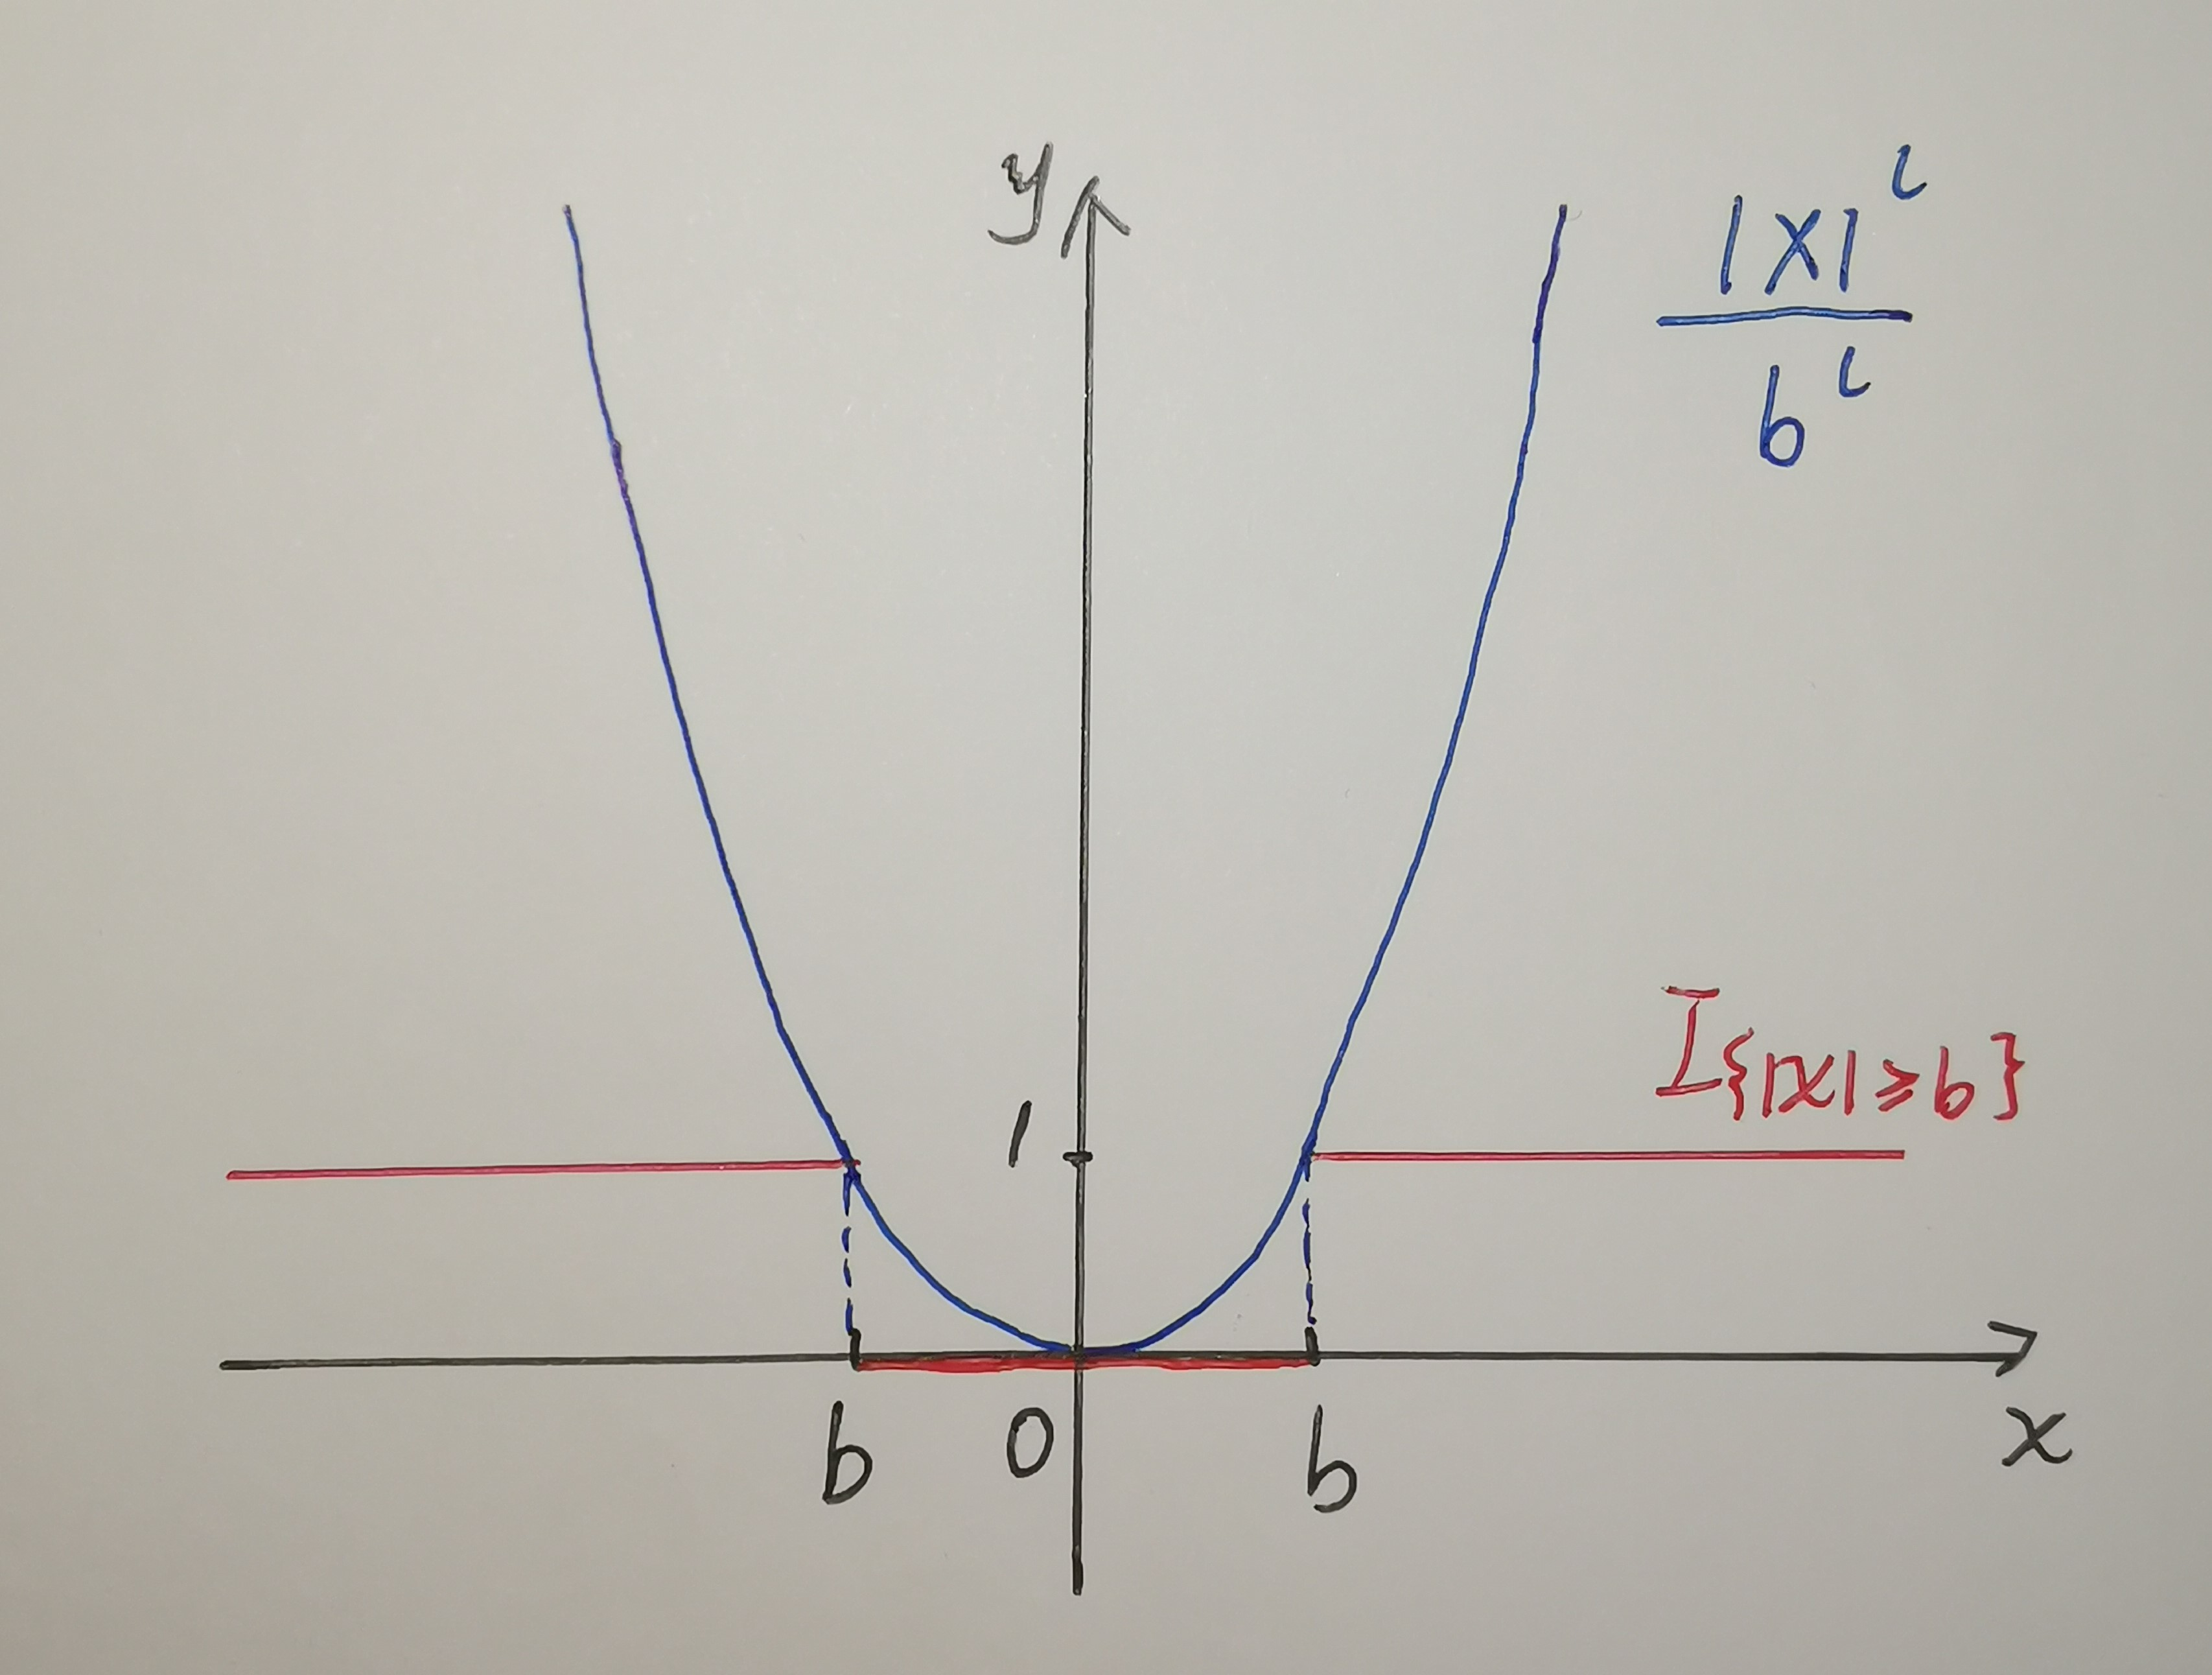
\includegraphics[width=0.8\linewidth]{l-markov.jpg}
    \caption{$l$阶马尔可夫不等式的几何直观}
    \label{fig:lmarkov}
\end{figure}

总之这个多项式曲线都会经过$(b,1)$这个点,所以说一定会有$l$阶Markov不等式成立。btw,从这个几何直观来讲,大家也应该能感受到,实际上这两个不等式都是相对较松的不等式。

\subsection*{Chebyshev不等式}
Chebyshev不等式是二阶Markov不等式的一种特殊情况,两者不是完全割裂的,相互对立却又相互统一。它将原点矩推广到中心矩,并对应地将期望替换为方差(因为一阶中心矩为零),是这样定义的,对于$\forall \varepsilon > 0$,有:
\begin{center}
    $P\{|X-\mu| \geq \varepsilon\} \leq \frac{\operatorname{Var}(X)}{\varepsilon^{2}}$
\end{center} \par

除了上述姚岑卓的解读,还有马同学以“年薪百万”做解读的\href{https://www.zhihu.com/question/27821324/answer/248693398}{切比雪夫不等式到底是个什么概念?},以及结合金融中布林带做解读的\href{https://www.zhihu.com/question/27821324/answer/92675490}{切比雪夫不等式到底是个什么概念?},我认为都是很好的直观理解。而至于记忆,其实我是这样记忆的,不等式中间这个小表情:
\begin{center}
    $\geq \varepsilon \leq$
\end{center} \par
实在是太可爱了!然后我就记住了……

\subsection{证明相合估计}
引入Markov和Chebyshev不等式后,我们就可以证明依概率收敛了。其实本质上这是一个大数定律问题,考研的同学不知道还能不能记起,当时我们其实是首先考虑拿辛钦大数定理证相合的,而研究生这里似乎只能考虑从这两个不等式证明就可以了。\par
所以诸君也必须清楚,本节内容要求大家对这两个不等式的熟练使用。对于这类题目,一般会要求证明一个统计量是相合估计,而无论是书中例题还是习题解答,直接就上Markov和Chebyshev不等式了,反正我第一眼看是有点蒙,但其实这一点是基于夹逼定理的。
\subsubsection{夹逼定理}
我们这里以Chebyshev为例,Markov类推,实际上我们可以对其扩写:
\begin{center}
    $0 \leq  P\{|X-\mu| \geq \varepsilon\} \leq \frac{\operatorname{Var}(X)}{\varepsilon^{2}}$
\end{center}
当“样本量足够大时”(即相合估计的基本思想,依概率收敛),进一步有:
\begin{center}
    $0 \leq \lim _{n \rightarrow \infty} P\{|X-\mu| \geq \varepsilon\} \leq \lim _{n \rightarrow \infty} \frac{\operatorname{Var}(X)}{\varepsilon^{2}}$
\end{center}

所以,如果我们能让最右式等于零,根据夹逼定理,就可以证明中间这个式子等于零,而这恰是相合估计的定义式。\par
这里给出\textbf{通过夹逼定理证明相合估计的基本步骤},假设统计量为$T$,待估参数函数为$q(\theta)$:
\begin{enumerate}
    \item 优先考虑一阶矩期望,即$E(T- q(\theta))$,如果这东西n趋于无穷的极限就为零,直接使用一阶Markov得证
    \item 若不为零,继续考虑二阶矩期望,如果这东西n趋于无穷的极限为零,使用二阶Markov得证
    \item 若还不为零,使用Chebyshev不等式(一二阶期望都计算出来了,方差就很好算了),若方差在n趋于无穷的极限为零,得证
    \item 若Chebyshev还做不出来,检查检查哪儿算错了,否则这题跳过吧……
\end{enumerate}

\subsubsection{补充定理}

除了使用夹逼定理,书上的定理2.4.1还给出了一种更进一步的方式,即一对相合估计的统计量和参数函数,再进一步取复合函数$g(·)$,如果这个复合函数连续,相合性仍然成立。所以这个算是一种“花拳绣腿”吧,实际上直接证出来就完了,一般不太使用,但还是提一嘴。\\\par

最后的最后,给出一个命题结束相合估计的内容。我们前边提到无偏估计和相合估计是个并列的概念,但实际上是有这一层关系的:「渐进无偏估计一定是相合估计」,可以想想如何证明。(提示:夫可尔马阶一)

\subsection{区间估计}

从区间估计开始,内容就变得逐渐有趣了。我们前边学过了(渐进)无偏、(渐进)有效、相合等内容,都是通过某个统计量来尝试估计一个未知参数的函数。而区间估计的思想,则是通过某一区间(或者说两个统计量)来作为参数的估计,即我们希望这个区间以\textbf{较大的概率}包含参数的真值。\par
那么到底是多大的概率呢?这就引入了置信度的概念,我们称,对于给定的$\alpha$,若有:
\begin{center}
    $P_{\theta}\left\{T_{1}\left(x_{1}, x_{2}, \cdots, x_{n}\right) \leqslant \theta \leqslant T_{2}\left(x_{1}, x_{2}, \cdots, x_{n}\right)\right\} \geqslant 1-\alpha$
\end{center} \par
则称这个$T_1$为\textbf{置信下限},$T_2$为\textbf{置信上限},$1-\alpha$为\textbf{置信水平}或\textbf{置信度}。\par
这个$\alpha$是一个磨人的小妖精,将会在接下来的内容中反复出现,大家可以留意一下。

\subsection{枢轴变量法}

所以这件事儿就可以和我们之前学过的「分位数」的概念联系起来,比如我们我设置置信下限是$\frac{\alpha}{2}$分位数,上限是$1-\frac{\alpha}{2}$分位数,这样一减不就是$1-\alpha$了吗,甚至在一些对称的分布中,这两个分位数还是互为相反数的,很美观。\par
于是科学家们很自然地想到,我们对四大分布研究得很透彻(书后附录从A到D,就是四大分布的分位数表),那么我们能否通过某些手段,将所研究的问题转化到四大分布上呢?这就是枢轴变量的由来(这个名字也很直观了)。而枢轴的选择,自然就是基于中心极限定理,或者在学习三大分布时的那些基本结论(参见第一篇数理统计学习笔记的2.4节内容)。\par
应注意,枢轴的选择必须是统计量(除了待估参数之外,\textbf{不能包含未知参数}),但同时我们又要本着\textbf{利用更多信息的原则},更好地选择枢轴。所谓利用更多信息,就是利用更多已知的参数。\\\par
\textbf{栗子1.}样本$x_1,x_2,\dots,x_n$来自某一正态总体$N(\mu,\sigma^2)$,$\sigma^2$\textbf{已知},求总体均值$\mu$的置信水平为$1-\alpha$的置信区间。\par
我们在此着重关注枢轴变量的选择,因为这个时候方差已知,所以就可以根据中心极限定理,使用$\frac{\bar{x}-\mu}{\sigma / \sqrt{n}} \sim N(0,1)$作为枢轴变量,构造一个标正态分布,通过样本均值来进行估计。也就是说,题目希望我们求一个:
\begin{center}
    $P\{T_{1} \leqslant \mu \leqslant T_{2}\} = 1-\alpha$
\end{center}
而实际上我们可以等价地变为:
\begin{center}
    $P\{\frac{\bar{x}-T_{1}}{\sigma / \sqrt{n}} \geqslant \frac{\bar{x}-\mu}{\sigma / \sqrt{n}} \geqslant \frac{\bar{x}-T_{2}}{\sigma / \sqrt{n}}\} = 1-\alpha$
\end{center} \par
而这是一个标正态,我们就可以像上边说的一样,比如选择$1-\frac{\alpha}{2}$分位数作为上限,$\frac{\alpha}{2}$分位数作为下限,在标正态中的分位数用$z$表示,也即令概率内部最左式为$z_{1-\frac{\alpha}{2}}$,最右式为$z_{\frac{\alpha}{2}}$,最终反解出$T_1$、$T_2$即可。\\\par
\textbf{栗子2.}样本$x_1,x_2,\dots,x_n$来自某一正态总体$N(\mu,\sigma^2)$,$\sigma^2$\textbf{未知},求总体均值$\mu$的置信水平为$1-\alpha$的置信区间。\par
因为此时$\sigma^2$\textbf{未知},我们就必须用样本方差$S^2$替换分布方差,而这个操作大家应该也已经轻车熟路了,我们知道$\frac{S}{\sigma}$可做为t分布的分母,自由度为$n-1$,于是只需要将例子1中的枢轴变量对$\frac{S}{\sigma}$作比,构造一个新的枢轴$\frac{\bar{x}-\mu}{S / \sqrt{n}} \sim t(1,n-1)$即可。此后的求解步骤在此略过,大家理解思想就好,书上也给了不少类似的习题供大家参阅。\\\par
最后还有一个问题就是,这种一边$1-\frac{\alpha}{2}$、一边$\frac{\alpha}{2}$的选择真的好吗?实际上这是「可信程度与精确度」之间一对不可调和的矛盾,对此Neyman表示,使区间平均长度尽可能短的这种方案是比较好的。也就是说,对于那些对称分布,尽量选取相反数的分位点作为上下限。不过总之,除非题目要求,大家无脑选择$1-\frac{\alpha}{2}$和$\frac{\alpha}{2}$这个组合总是没错的。\\\par
总结而言,枢轴变量法求解区间估计的基本步骤就是:
\begin{enumerate}
    \item 寻找信息尽可能多的枢轴
    \item 对置信上下限做同样的变换,得到一个枢轴分布的概率表达式
    \item 对应取分位数(一般为$1-\frac{\alpha}{2}$和$\frac{\alpha}{2}$),反解得到置信上下限
\end{enumerate}

以上,有关\textbf{参数估计}的内容就完结了。

\section{假设检验初步}
作业内容参考:3.2、3.4(韦卫老师留的是3.1、3.3)\par
因为一些特殊的原因,本次课我是在韦卫老师班上的。目前单次观察得到的结论时,韦老师激情有余而不得要领,孙老师则往往是鞭辟入里而波澜不惊,要是这两个老师能结合结合就好了……

\subsection{参数估计与假设检验}
进入本节内容前,我们必须明白第二章参数估计与第三章假设检验的关系。通俗地解释,参数估计是希望从观测样本的一些统计量,去逼近、近似或估计参数(的函数);而假设检验就像是在其对立面,是先假设参数已知,再抽样验证我的假设成立与否(接受还是拒绝)。\par
所以说假设检验更像是“假说演绎法”,也更加偏向应用一些,在生活中我们也常常需要做出这样的回答,比如说双十一买了十包洗衣粉,标称100g,然而每一包都只有50g,那么你肯定就会做出一个假设“我被骗了”,或者说“这些洗衣粉有问题”,这种我们希望去验证的假设被称为\textbf{原假设$H_0$}。在假设检验中,我们一般认为,原假设不成立、即拒绝原假设,就意味着接受了\textbf{备择假设}。However,大家需要注意这两者是\textbf{互斥}关系,但却不是\textbf{对立}关系。\par

举一个几乎所有老师都会举的例子,大家要对这个例子牢记于心、反复咀嚼。比如我去看病,此时原假设与备择假设就应该是:
\begin{center}
    $H_0$:我有病,~~$H_1$:我没病
\end{center} \par
像这种是非判断,参数空间是二值的(未知参数就是有没有病,要么有要么无),此时我们称其为\textbf{简单假设}。\par
再举一个例子,比如我是老师、你们是学生,我判断你们也就是80分的水平(考个试你们的平均分大概在80分左右,这个“左右”的心理预期限定在70-90分吧),而我的备择假设是90分(“左右”的心理预期限定在80-100分),这个时候参数就不是二值的了,我们就称这样的假设检验是\textbf{复合假设}。一般来讲,多数假设检验问题都是复合假设。\par

\subsection{拒绝域、接受域}
更进一步,我们不妨定义一些术语来描述这种“左右”、心理预期这样的模糊说法,这就是拒绝域与接受域。一般来讲,我们在进行假设检验活动的时候,是\textbf{希望原假设不成立}的,比如我去看病,这时我们做的原假设是我有病,实际上我是不希望自己有病的;比如我买了洗衣粉,我怀疑这个洗衣粉有问题,但其实我是希望他没问题的。所以总的来说,在Everything's fine的时候我们就没必要假设检验了嘛——于是乎,我其实更关心我什么时候拒绝这个事情。\par
所以我们可以将样本空间划分为两个互不相交的部分,定义$W$和$W^c$分别表示\textbf{拒绝域}和\textbf{接受域},当$(x_1,\dots,x_n) \in W$时拒绝$H_0$,\textbf{并}接受$H_1$;当$(x_1,\dots,x_n) \in W^c$时接受$H_0$。\par
这里基本是书上的原话,其实有两件事情我认为没有定义清楚,在此做补充说明:
\begin{enumerate}
    \item 什么叫$(x_1,\dots,x_n) \in W$?
    \item 拒绝域与接受域是否是对立的,也就是其并集是否是整个样本空间?$H_0$的拒绝域是否就是$H_1$的接受域?
\end{enumerate} \par
对于第一点,嗯,其实这个地方往往是题目给你下套的地方。这个拒绝域是人为定义的,比如你可以认为“班里的同学\textbf{都}考到70-90分才接受,就算有个人考100分也拒绝”,也可以定义比如“平均分介于70-90分之间就行”,但是题目就不会这么善良了,动不动就来个什么样本求和大于等于3之类的,这个时候就要涉及什么分布可加性之类的东西,要求解具体的拒绝域大小,也就是后面要说的“势”。\par
对于第二点,我这里认为的是:拒绝域与接受域相互对立,但是$H_0$和$H_1$各自有自己的拒绝域。书上说“给定一个检验,其实等价于给定其拒绝域”,以及韦卫老师不断强调“如果把原假设和备择假设交换,这就是完全不同的两码事儿了”,所以你细品,这意思应该就是说:交换$H_0$和$H_1$意味着$W$和$W^c$的改变,但不一定意味着互换(确实就是两码事儿了)。关于这一点大家可以参照前边关于考试成绩的例子进一步理解。

\subsection{第I、II类错误、势、势函数}

接下来以有病没病这个例子来给出第一类错误、第二类错误和势的概念。以我的理解,势并不是什么奇怪的东西,可能是受考研只学第一类第二类错误的影响,以及定义了什么$\gamma$、$g$的乱七八糟,我一开始对势的理解很不好,其实势应该是跟第一类错误、第二类错误并列的东西,我们这里结合\textbf{「机器学习」}(是的,他居然和机器学习联系起来了)中的相关知识来一道把这个东西讲清楚。

\textbf{一个非常经典的栗子.}考虑病人看病问题,有如下假设:
\begin{center}
    $H_0$:病人有病,~~$H_1$:病人没病
\end{center} \par
\begin{enumerate}
    \item 如果$H_0$\textbf{真的}成立,同时我又在假设检验中\textbf{接受了$H_0$},那么这是一件天大的好事儿——病人真的有病,我还给他看出来了,那不是好事儿是啥!\par {\textcolor{violet}{这对应着机器学习中的True Positive(TP,真正例)样本}}。
    \item 如果$H_0$\textbf{真的}成立,但我又在假设检验中\textbf{拒绝了$H_0$},那么这是一件比较坏的事儿——病人真的有病,我却没给他看出来,那这个病人有点惨。我们称这样的事情叫做\textbf{第一类错误},也叫“弃真”,记为$\alpha$。\par {\textcolor{violet}{这对应着机器学习中的False Negative(FN,假反例)样本}}。
    \item 如果$H_0$\textbf{真的不}成立,并且在看病这样一个二值事件中意味着$H_1$\textbf{真的}成立,但我又在假设检验中\textbf{接受了$H_0$},那么这是一件没那么坏的事儿——病人其实没病,我却误诊认为他有病,那这个病人顶多就是多吃点儿药,一般也没啥大问题。我们称这样的事情叫做\textbf{第二类错误},也叫“取伪”,记为$\beta$。\par {\textcolor{violet}{这对应着机器学习中的False Positive(FP,假正例)样本}}。
    \item 如果$H_0$\textbf{真的不}成立,并且在看病这样一个二值事件中意味着$H_1$\textbf{真的}成立,同时我又在假设检验中\textbf{拒绝了$H_0$},那么这是一件也挺不错的的事儿——病人其实没病,我也认为他没病,那就是个杞人忧天罢了。我们称这样的事情叫做\textbf{势}(Power),记为$\gamma$。\par {\textcolor{violet}{这对应着机器学习中的True Negative(TN,真反例)样本}}。
\end{enumerate}

\begin{figure}[H]
    \centering
    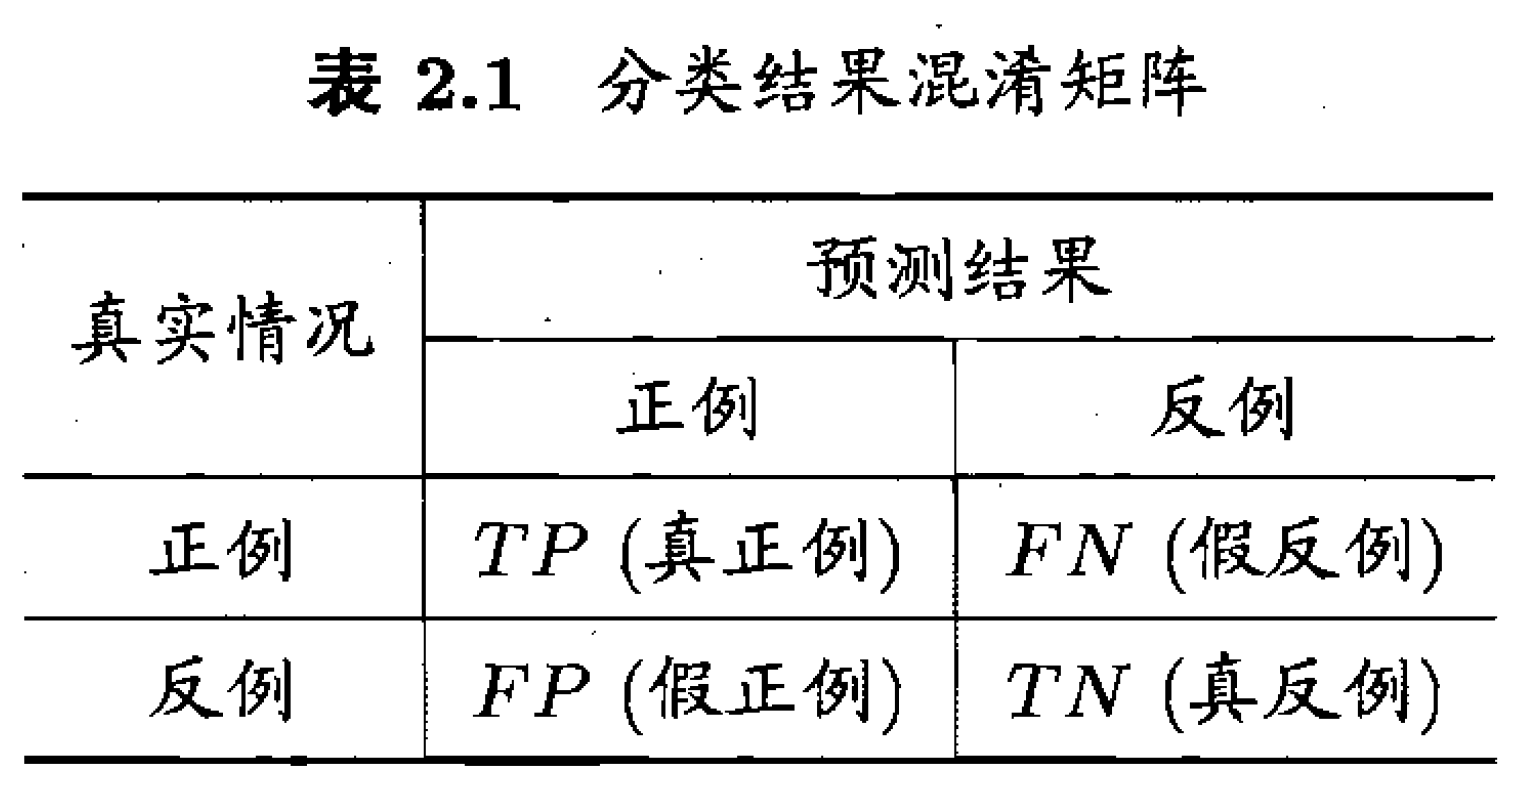
\includegraphics[width=0.5\linewidth]{confusion.png}
    \caption{二分类问题的混淆矩阵(confusion matrix)~from西瓜书}
    \label{fig:confusioin}
\end{figure}

无论是从混淆矩阵中,还是从定义本身,我们都可以很轻易得到归一性:\par
\begin{enumerate}
    \item 我们虽然没有定义“天大的好事儿”叫什么,但它的概率应该是$1-\alpha$,即和第一类错误成对立面。
    \item 第二类错误与势也是一个对立面,应该有$\beta+\gamma=1$。
\end{enumerate}\par
理解以上两点时,只需要把$H_0$成立或不成立当做一个大前提、拒绝与接受当成一个小前提,小前提需要归一就理解了。\par 
另外注意,书上似乎倾向于使用$\alpha(\theta)$、$\beta(\theta)$等(其中$\theta$是未知参数)这样的写法,我个人认为这样的说法其实不好,毕竟$\alpha$和$\beta$的取值其实只能分别关于原假设和备择假设(的参数)。这样的写法可能主要是针对于之后要定义的势函数$g(\theta)$而言。\par
在机器学习中,我们知道\textbf{查全率}(Precision)与\textbf{查准率}(Recall)是一对不可调和的矛盾,想要同时提升查全率与查准率很难,这两个概念定义为:
\begin{center}
    $P=\frac{TP}{TP+FP}$,$R=\frac{TP}{TP+FN}$
\end{center} \par
对应在看病的例子中,实际上查准率的含义就是:在所有判了有病的样例中,我们尽量减少误判;而查全率的含义就是,对于所有有病的样例,我们尽量地把它们都查出来,尽量不出现漏网之鱼。\par
想要提升查准率,就要减小第二类错误(没病被判有病);想要提升查全率,就要减小第一类错误(有病却没查出来),所以\textbf{本质上查全率与查准率这对矛盾不可调和的原因,其实是因为第一类错误与第二类错误难以同时减小}!\par

如果非要在第一类错误和第二类错误中选择谁更严重,那么应该是第一类错误更严重一些(有病没看出来肯定比多吃药惨)。于是这就引出了\textbf{Neyman-Pearson检验}的思想,即第一类错误更加重要一些,那么我们就在第一类错误的允许范围内尽量减小第二类错误发生的概率,这是解决二者矛盾的普遍做法。\par
所以从这个角度讲,“宁可错杀三千,不可放过一个”还是有那么一些道理的,然而问题可能就出在三千这个量有点多,第一类错误太小第二类错误太大,这并不符合Neyman-Pearson检验的原则,哎,你说这汪精卫手底下怎么就没个数理统计学家呢。(笑)\par

最后我们应该认识到,在样本容量固定的情况下,$\alpha$和$\beta$呈此消彼长的状态;提升样本容量的大小可以同时降低二者,甚至在样本容量充分大的时候可以将两类错误缩小到任意小。

我们继续给出势函数的定义:书上把“一个检验\textbf{犯第一类错误的概率}和\textbf{势}”定义为势函数,这个函数还是个风马牛不相及的符复合分段函数:

\begin{center}
    $
    g(\theta)=\left\{
    \begin{aligned}
    \alpha(\theta),~ & \theta \in \Theta_{0} \\
    \gamma(\theta),~ & \theta \in \Theta_{1}
    \end{aligned}\right.$
\end{center} \par
(顺便强调一下,$\gamma(\theta)$也可以写成$1-\beta(\theta)$)\par
所以我觉得这个挺扯的,其实更直观的定义应该是“无论哪个假设真正成立,拒绝它的可能性”,那么这样的定义当然是要根据哪个假设成立分别讨论了,而原假设成立拒绝这意味着第一类错误、备择假设成立拒绝这意味着势,这样我认为就更直观清晰了。这就是\textbf{势函数},也叫\textbf{功效函数}。\\ \par
\subsection{习题与讨论}
最后,我必须极度驳斥一下本次作业习题详解,以及一些书上例题中的相关解答。既然势函数如此定义了,怎么能就答个$g(p)$、$g(\lambda)$(作业3.1、作业3.2)而不做分段讨论呢。虽然说势函数的本质就是拒绝一个假设的概率,关于参数的函数,然而参数的取值空间实际上是离散甚至二值的,既然书上那样定义了我认为解答就应该保持一致性。\par
我们就以作业3.1作为本节内容的结束,在总结做题套路的同时强化一下以上的相关概念。\par
\textbf{习题3.1}设总体$X$服从两点分布$B(1,p)$,$x1,x2,x3$是来自总体$X$的简单样本,考虑假设检验问题
设检验问题
\begin{center}
    $H_0:p=\frac{1}{2}$,~~$H_1:p=\frac{3}{4}$
\end{center} 
若取拒绝域$W=\left\{\left(x_{1}, x_{2}, x_{3}\right): x_{1}+x_{2}+x_{3} \geqslant 1\right\}$,求势函数,犯第一类错误和第二类错误的概率以及势。\\\par
1.首先求拒绝事件的概率(实际上就是势函数)。\par
$x_{1}+x_{2}+x_{3}$服从$B(3,p)$,故有$P(x_{1}+x_{2}+x_{3} \geqslant 1) = 1-P(x_{1}+x_{2}+x_{3} = 0)=1-(1-p)^3$,也即,当两点分布的概率为p时,参数\textbf{落入}拒绝域的概率为$1-(1-p)^3$。\par
2.其次写出势函数(帮助理清思路),按照我的理解应该这样写:\par
\begin{center}
    $
    g(\theta)=\left\{
    \begin{aligned}
    \alpha(\theta),~ & p \in \Theta_{0} & (p=\frac{1}{2}) \\
    \gamma(\theta),~ & p \in \Theta_{1} & (p=\frac{3}{4})
    \end{aligned}\right.$
\end{center} \par
3.代入两个假设中的参数到1.中所求概率,求解第一类概率和势,写出完整势函数:\par $\alpha(\frac{1}{2}) = 1-(1-\frac{1}{2})^3 = \frac{7}{8}$,$\gamma(\frac{3}{4}) = 1-(1-\frac{3}{4})^3 = \frac{63}{64}$,终而写出势函数:
\begin{center}
    $
    g(\theta)=\left\{
    \begin{aligned}
    \frac{7}{8},~ & p \in \Theta_{0} & (p=\frac{1}{2}) \\
    \frac{63}{64},~ & p \in \Theta_{1} & (p=\frac{3}{4})
    \end{aligned}\right.$
\end{center} \par
4.计算第二类错误概率,也即势的反面$1-\gamma(p)$:$\beta(p)=1-\frac{63}{64} = \frac{1}{64}$ 。\par
5.整理作答。


\subsection{$\alpha$的三种身份}
最后我们来对$\alpha$这个磨人的小妖精做一个总结。我个人认为它的身份有三个:
\begin{enumerate}
    \item 在参数估计(区间估计)中,它是分位数,关系着置信水平、置信度。
    \item 在假设检验中,也是第一类错误。
    \item 在Neyman-Pearson假设检验中,也被称作显著性。
\end{enumerate}\par
关于这个$\alpha$我认为大家也不要太在意,遇到题目了,具体问题具体分析即可。
\end{document}